\documentclass[9pt,aspectratio=169,xcolor=table]{beamer}

%~~~~~~~~~~~~~~~~~~~~~~~~~~~~~~~~~~~~~~~~~~~~~~~~~~~~~~~~~~~~~~~~~~~~~~~~~~~~~~
% Use roboto Font (recommended)
\usepackage[sfdefault]{roboto}
\usepackage[utf8]{inputenc}
\usepackage[T1]{fontenc}
%~~~~~~~~~~~~~~~~~~~~~~~~~~~~~~~~~~~~~~~~~~~~~~~~~~~~~~~~~~~~~~~~~~~~~~~~~~~~~~

%~~~~~~~~~~~~~~~~~~~~~~~~~~~~~~~~~~~~~~~~~~~~~~~~~~~~~~~~~~~~~~~~~~~~~~~~~~~~~~
% Define where theme files are located. ('/styles')
\usepackage{styles/fluxmacros}
\usefolder{styles}
% Use Flux theme v0.1 beta
% Available style: asphalt, blue, red, green, gray
\usetheme[style=gray]{flux}
%~~~~~~~~~~~~~~~~~~~~~~~~~~~~~~~~~~~~~~~~~~~~~~~~~~~~~~~~~~~~~~~~~~~~~~~~~~~~~~

%~~~~~~~~~~~~~~~~~~~~~~~~~~~~~~~~~~~~~~~~~~~~~~~~~~~~~~~~~~~~~~~~~~~~~~~~~~~~~~
% Extra packages
\usepackage{booktabs}
\usepackage{colortbl}
\usepackage{ragged2e}
\usepackage{amssymb}
\usepackage{multirow}
\usepackage{tikz}
\usetikzlibrary{arrows.meta, positioning, fit, backgrounds, calc, decorations.pathreplacing}
\setbeamertemplate{itemize items}[square]
\usepackage[scaled=.92]{beramono}
\usepackage{listings}
\usepackage{styles/lstlangarm}
\usepackage{array}
\definecolor{bgcolor}{HTML}{F2E9E9}
% lstlangarm.sty references \color{mauve} for string literals but never defines
% it -- only fires when a listing contains a string. Define it here.
\definecolor{mauve}{rgb}{0.58,0,0.82}
% lstlangarm's C style sets commentstyle=green!20, which is unreadable on the
% pink listing background. Darken it globally.
\lstset{commentstyle=\color{green!45!black}}
% ragged-right fixed-width column -- must be defined in the preamble, never
% inside a frame (\newcolumntype's #1 breaks beamer's frame scanner)
\newcolumntype{R}[1]{>{\RaggedRight\arraybackslash}p{#1}}
%~~~~~~~~~~~~~~~~~~~~~~~~~~~~~~~~~~~~~~~~~~~~~~~~~~~~~~~~~~~~~~~~~~~~~~~~~~~~~~
% Table striping: odd rows white, even rows very light gray.
% Needs \documentclass[...,xcolor=table]{beamer} (beamer loads xcolor itself,
% so the option must go on the class, not \usepackage).
\definecolor{stripe}{gray}{0.94}
% \striped makes body rows alternate white, gray, white, ... starting white.
% \rowcolors counts from the first coloured body row; the header is not counted.
\newcommand{\striped}{\rowcolors{1}{white}{stripe}}
%~~~~~~~~~~~~~~~~~~~~~~~~~~~~~~~~~~~~~~~~~~~~~~~~~~~~~~~~~~~~~~~~~~~~~~~~~~~~~~

%~~~~~~~~~~~~~~~~~~~~~~~~~~~~~~~~~~~~~~~~~~~~~~~~~~~~~~~~~~~~~~~~~~~~~~~~~~~~~~
% TikZ block styles -- matches ch1/ch2
% Colour variables are named identically in the book's stm32primer.tex, so any
% tikzpicture using only the \tikzset{...} styles below can be copied verbatim
% between slides and book. Only the \definecolor/\colorlet VALUES differ: the
% book is printed, so it keeps every stroke pure black with muted fills. These
% slides are projected, so both fill AND stroke are bright and saturated to
% grab attention -- see stm32primer.tex for the print palette.
\definecolor{blkfill}{HTML}{DCEBFF}
\definecolor{blkline}{HTML}{1565C0}
\definecolor{accentfill}{HTML}{FFE0B2}
\definecolor{accentline}{HTML}{E65100}
\definecolor{memfill}{HTML}{DFF5DA}
\definecolor{memline}{HTML}{2E7D32}
\definecolor{cellfill}{HTML}{FFFFFF}
\definecolor{cellline}{HTML}{424242}
\definecolor{bitmaskfill}{HTML}{DCEBFF}
\definecolor{bitmaskline}{HTML}{1565C0}
\definecolor{bithitfill}{HTML}{FFE0B2}
\definecolor{bithitline}{HTML}{E65100}
\tikzset{
  blk/.style   = {rectangle, rounded corners=2pt, draw=blkline, fill=blkfill,
                  thick, align=center, font=\small, minimum height=9mm, inner sep=3pt},
  cpublk/.style= {rectangle, rounded corners=2pt, draw=accentline, fill=accentfill,
                  thick, align=center, font=\small\bfseries, minimum height=9mm, inner sep=3pt},
  memblk/.style= {rectangle, rounded corners=2pt, draw=memline, fill=memfill,
                  thick, align=center, font=\small, minimum height=9mm, inner sep=3pt},
  cell/.style  = {rectangle, draw=cellline, fill=cellfill, align=center,
                  font=\normalsize\ttfamily, minimum height=7mm, inner sep=2pt},
  lbl/.style   = {font=\scriptsize, text=Gray},
  flow/.style  = {-{Stealth[length=2mm]}, thick, draw=blkline},
  busline/.style={thick, draw=cellline},
}
% NOTE (theme quirks -- all fail SILENTLY, always page through the PDF):
%  - a second \\ inside a nested {...} group in a TikZ node breaks parsing
%  - {\small ...} wrapped around a nested itemize eats the frame title + list
%  - \usebeamercolor on a [plain] frame falls through to an unstyled default
%  - \newcolumntype inside a frame breaks beamer's frame scanner
%  - lstlisting needs \begin{frame}[fragile]
%  - a TikZ picture wider than its column silently overflows into neighbours
%~~~~~~~~~~~~~~~~~~~~~~~~~~~~~~~~~~~~~~~~~~~~~~~~~~~~~~~~~~~~~~~~~~~~~~~~~~~~~~

%%%%%%%%%%%%%%%%%%%%%%%%%%%%%%%%%%%
%% BEGIN CONDITIONAL COMPILATION %%
%%%%%%%%%%%%%%%%%%%%%%%%%%%%%%%%%%%
\newif\ifwebex
%\webextrue % uncomment to generate section separator
\ifwebex
\AtBeginSection[]{
  \begin{frame}
  \vfill
  \centering
  \begin{beamercolorbox}[sep=8pt,center,shadow=true,rounded=true]{title}
    \usebeamerfont{title}\insertsectionhead\par%
  \end{beamercolorbox}
  \vfill
  \end{frame}
}
\else
\AtBeginSection[]
{
{
    \setbeamercolor{background canvas}{bg=yellow!10}
    \begin{frame}[plain]
        \frametitle{Table of Contents}
        \tableofcontents[currentsection]
    \end{frame}
}
}
\fi
%%%%%%%%%%%%%%%%%%%%%%%%%%%%%%%%%%%
%% END CONDITIONAL COMPILATION   %%
%%%%%%%%%%%%%%%%%%%%%%%%%%%%%%%%%%%

%~~~~~~~~~~~~~~~~~~~~~~~~~~~~~~~~~~~~~~~~~~~~~~~~~~~~~~~~~~~~~~~~~~~~~~~~~~~~~~
% Information
\title{Memory, Addressing and Pointers}
\subtitle{\emph{Introduction to ARM Cortex-M Microprocessors} --- Chapter 3}
\author{Mun\'{i}m Zabidi}
\institute{\color{primary}Faculty of Electrical Engineering, Universiti Teknologi Malaysia}
\date{\today}
\titlegraphic{assets/logoutmwhite.png}
%~~~~~~~~~~~~~~~~~~~~~~~~~~~~~~~~~~~~~~~~~~~~~~~~~~~~~~~~~~~~~~~~~~~~~~~~~~~~~~

\begin{document}

\titlepage

%===============================================================================
\section{Why This Matters}
%===============================================================================

\begin{frame}{Why This Chapter Matters}
    \begin{columns}[T]
    \begin{column}{.47\textwidth}
        {\normalsize A microcontroller has no instruction that means ``turn on the LED''. It only reads and writes numbered locations. So hardware control becomes one question: \emph{which number do I write, and to which address?} This chapter links the C you know to the addresses the processor uses. It is the shortest path from \texttt{int x;} to \texttt{GPIOA->ODR}.}
    \end{column}
    \begin{column}{.51\textwidth}
        \begin{block}{After this chapter, you can:}
        {\small
        \begin{enumerate}\itemsep2pt
            \item Explain an address, and how it differs from its contents.
            \item Use \texttt{\&} and \texttt{*}.
            \item Give the size of a byte, halfword and word; compute an array element's address.
            \item Choose the correct fixed-width type.
            \item Explain what \texttt{const} and \texttt{volatile} do to generated code.
            \item Write a pointer that reads and writes a hardware register.
        \end{enumerate}}
        \end{block}
    \end{column}
    \end{columns}
\end{frame}



%===============================================================================
\section{Memory and Addresses}
%===============================================================================

\begin{frame}{Memory Is a Numbered Array of Bytes}
	\leavevmode
	Memory is organized as a sequence of one-byte locations. Each byte has
	a unique \alert{address}, which acts as its location number.

	\vspace{3mm}
	A 32-bit address can identify
	\[
	2^{32} = 4{,}294{,}967{,}296
	\]
	different byte locations.

	\vspace{2mm}
	\begin{center}
		{\small
			\begin{tabular}{@{}ll@{}}
				\textbf{Address}   & \emph{where} a byte is located \\[1mm]
				\textbf{Contents}  & \emph{what} is stored at that location
		\end{tabular}}
	\end{center}

	\vspace{3mm}
	\begin{block}{Keep these two apart}
		A house number and the family living in it are different things.
		An address identifies a location; it is not the value stored there.
	\end{block}
\end{frame}

\begin{frame}{Storing a Word}
	\leavevmode

	\begin{columns}[c]
		\begin{column}{.48\textwidth}
			{\small
				A 32-bit word is stored in memory starting at 0x2000 looks like this:			}

			\vspace{2mm}
			\begin{center}

				\begin{tabular}{|c|c|}
					\hline
					\textit{Address} & \textit{Contents} \\
					\hline
					0x2000 & 0xDE \\
					\hline
					0x2001 & 0xC0 \\
					\hline
					0x2002 & 0xAD \\
					\hline
					0x2003 & 0xDE \\
					\hline
				\end{tabular}

			\end{center}
		\end{column}

		\begin{column}{.46\textwidth}
			{\small
				Notice that the addresses increase by one because memory is
				\alert{byte-addressable}: each address identifies one byte.

				\vspace{3mm}

				A larger value occupies several consecutive byte locations.
				For example, a 32-bit word occupies four bytes.

				\vspace{3mm}

				So, an address identifies the \emph{first byte} of a
				multi-byte object. The remaining bytes follow at the
				next addresses.
			}
		\end{column}
	\end{columns}
\end{frame}

\begin{frame}{A Variable Has an Address}
	\leavevmode

	Suppose \texttt{uint32\_t x = 42;} and the compiler puts \texttt{x} at
	\texttt{0x20000100}. We can ask two different questions:

	\vspace{3mm}
	\begin{center}
		{\small
			\begin{tabular}{@{}ll@{}}
				\emph{Where does \texttt{x} live?}
				& \texttt{0x20000100} --- the \textbf{address} \\[1mm]
				\emph{What value does \texttt{x} contain?}
				& \texttt{42} --- the \textbf{value}
		\end{tabular}}
	\end{center}

	\vspace{3mm}
	{
		In C, \texttt{x} names the value, while \texttt{\&x} produces its
		address.
	}
    \vspace{3mm}
	\begin{block}{You already know this from digital electronics}
		An address is the input to a
		\alert{decoder}. With memory-mapped I/O, the decoder can select
		peripheral registers as well as RAM locations.
	\end{block}

\end{frame}

%===============================================================================
\section{Pointers}
%===============================================================================

\begin{frame}[fragile]{A Pointer Holds an Address}{A variable whose value is an address}
    \leavevmode
    We just saw that \texttt{\&x} gives the address where \texttt{x} lives.
    C needs somewhere to \alert{keep} that address. A \textbf{pointer} is a
    variable built for exactly this job.

    \vspace{2mm}
    \begin{columns}[T]
    \begin{column}{.48\textwidth}
        \begin{itemize}
            \item \texttt{\&x} --- \alert{address-of}: the address at which
                  \texttt{x} is stored
            \item \texttt{*p} --- \alert{dereference}: the value stored at the
                  address held in \texttt{p}
        \end{itemize}
        \vspace{1mm}
        {\small These two undo each other: \texttt{*(\&x)} is just
        \texttt{x}.}
    \end{column}
    \begin{column}{.48\textwidth}
\begin{lstlisting}[language=C, basicstyle=\ttfamily\footnotesize]
uint32_t  x = 42;
uint32_t *p = &x;   // p holds x's
                    // ADDRESS
uint32_t v = *p;    // v becomes 42
*p = 99;            // x becomes 99
\end{lstlisting}
    \end{column}
    \end{columns}

    \vspace{2mm}
    \begin{center}
    \begin{tikzpicture}[x=11mm, y=9mm]
        \node[lbl] at (-1.1,1.7) {\textit{Address}};
        \node[lbl] at (0.4,1.7)  {\textit{Name}};
        \node[lbl] at (2.0,1.7)  {\textit{Contents}};
        \node[lbl, anchor=east, font=\footnotesize\ttfamily] at (-0.4,1) {0x20000100};
        \node[cell, minimum width=11mm] (nx) at (0.4,1) {x};
        \node[cell, minimum width=28mm] (vx) at (2.0,1) {42};
        \node[lbl, anchor=west] at (3.5,1) {the value};
        \node[lbl, anchor=east, font=\footnotesize\ttfamily] at (-0.4,-0.5) {0x20000104};
        \node[cell, minimum width=11mm] (np) at (0.4,-0.5) {p};
        \node[cell, minimum width=28mm, draw=secondary, fill=secondary!12]
             (vp) at (2.0,-0.5) {0x20000100};
        \node[lbl, anchor=west, align=left] at (3.5,-0.5) {an address,\\not a value};
        \draw[flow] (vp.north) -- (vx.south);
    \end{tikzpicture}
    \end{center}
\end{frame}

\begin{frame}{Arrays Are Address Arithmetic}
    \begin{columns}[c]
    \begin{column}{.46\textwidth}
        \begin{center}
        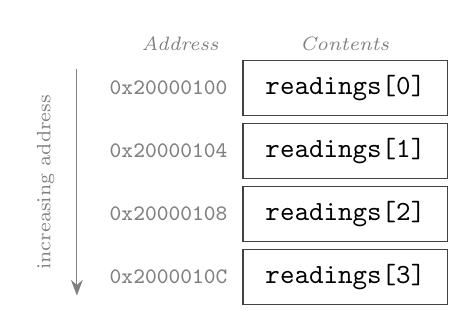
\begin{tikzpicture}[x=11mm, y=8mm]
            \node[lbl] at (-1.15,3.7) {\textit{Address}};
            \node[lbl] at (0.75,3.7)  {\textit{Contents}};
            \foreach \i/\addr in {0/0x20000100, 1/0x20000104, 2/0x20000108, 3/0x2000010C}{
                \pgfmathsetmacro{\y}{3-\i}
                \node[cell, minimum width=26mm] (c\i) at (0.75,\y) {readings[\i]};
                \node[lbl, anchor=east, font=\footnotesize\ttfamily] at (-0.5,\y) {\addr};
            }
            \draw[-{Stealth[length=2mm]}, draw=Gray] (-2.35,3.3) -- (-2.35,-0.3);
            \node[lbl, anchor=south, rotate=90] at (-2.5,1.5) {increasing address};
        \end{tikzpicture}
        \end{center}
    \end{column}
    \begin{column}{.5\textwidth}
        An array is a block of \alert{elements}, placed one after another,
        all the same size. So its addresses follow a formula.

        \vspace{3mm}
        \begin{center}
        \fbox{\parbox{.92\textwidth}{\centering\small\vspace{1mm}
        address of element $i$ $=$ \\ base $+$ ($i$ $\times$ element size)
        \vspace{1mm}}}
        \end{center}

        \vspace{2mm}
        {\small For \texttt{readings[2]}: \texttt{0x20000100} $+ (2 \times 4) =$
        \alert{\texttt{0x20000108}}.}

        \vspace{2mm}
        {\small The processor can perform this scaling as part of the
        memory access instruction.}
    \end{column}
    \end{columns}
\end{frame}

\begin{frame}[fragile]{Pointer Arithmetic}
    \leavevmode
    A pointer already holds an address. Adding an integer to it moves that
    address by \alert{whole elements}, not by bytes --- because the
    pointer's type tells C how large one element is.

    \vspace{2mm}
    \begin{columns}[T]
    \begin{column}{.5\textwidth}
\begin{lstlisting}[language=C, basicstyle=\ttfamily\footnotesize]
uint32_t *p = &readings[0];
              // p = 0x20000100
p + 1;        // 0x20000104  (+4)
p + 2;        // 0x20000108

uint8_t *q = (uint8_t *)p;
q + 1;        // 0x20000101  (+1)
\end{lstlisting}
    \end{column}
    \begin{column}{.46\textwidth}
        The compiler uses the array formula. It gets the element size
        from the \alert{pointer's own type}.

        \vspace{3mm}
        \begin{center}
        \texttt{p[i]} \quad$\equiv$\quad \texttt{*(p + i)}
        \end{center}

        \vspace{2mm}
        {\small Array indexing \emph{is} pointer arithmetic.}
    \end{column}
    \end{columns}

    \vspace{2mm}
    \begin{block}{Where you will meet this}
        CMSIS declares the GPIO alternate-function registers as
        \texttt{AFR[2]}. These are two fixed hardware registers. But
        because indexing is pointer arithmetic, \texttt{GPIOA->AFR[1]}
        computes the right address by itself.
    \end{block}
\end{frame}

\begin{frame}{Three Sentences to Remember}
    \leavevmode
    So far, three ideas are enough to explain how C reaches an address of
    its choosing. Learn these; everything else in this chapter builds on
    them:

    \vspace{4mm}
    \begin{center}
    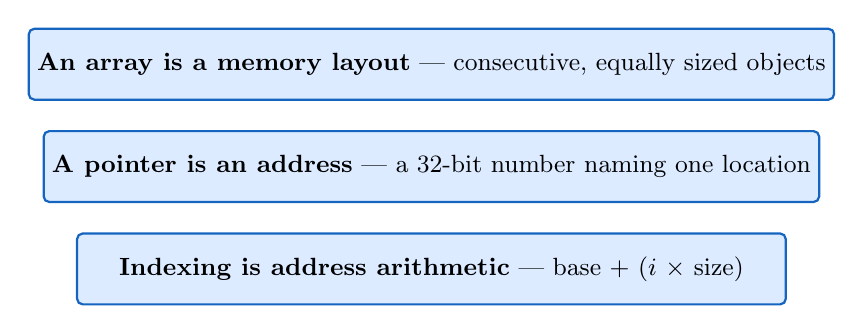
\begin{tikzpicture}[x=10mm, y=13mm]
        \node[blk, minimum width=90mm, minimum height=9mm] (a) at (0,2) {\textbf{An array is a memory layout} --- consecutive, equally sized objects};
        \node[blk, minimum width=90mm, minimum height=9mm] (b) at (0,1) {\textbf{A pointer is an address} --- a 32-bit number naming one location};
        \node[blk, minimum width=90mm, minimum height=9mm] (c) at (0,0) {\textbf{Indexing is address arithmetic} --- base $+$ ($i$ $\times$ size)};
    \end{tikzpicture}
    \end{center}

    \vspace{2mm}
    {\small There is no fourth idea hiding here. A \texttt{struct},
    seen later, is just a layout whose elements have different sizes.
    A peripheral register block, later still, is just a struct whose
    base address is fixed by the chip, not chosen by the compiler.
    Next: \alert{where do these addresses actually lead?}}
\end{frame}

%===============================================================================
\section{The Memory Map}
%===============================================================================

\begin{frame}{Where Those Addresses Lead}
	\leavevmode

	\begin{columns}[c]
		\begin{column}{.46\textwidth}
			{\small
				A Cortex-M microcontroller splits its 4\,GB address space
				into a few large regions:
			}

			\vspace{2mm}
			\begin{center}
				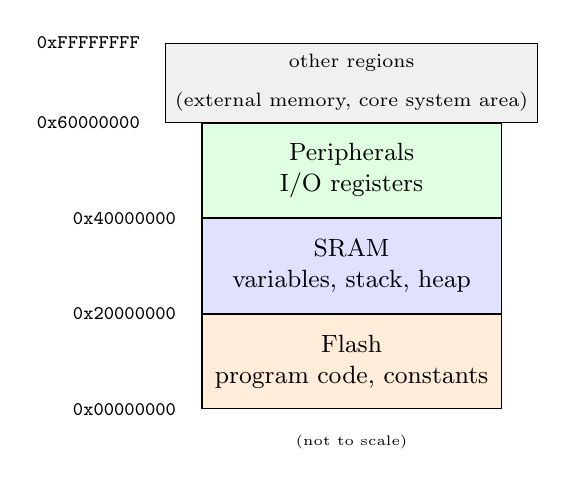
\begin{tikzpicture}[
					x=1mm, y=1mm,
					block/.style={
						draw, minimum width=38mm, align=center, font=\small
					},
					addrlbl/.style={font=\scriptsize\ttfamily}
					]
					\node[block, minimum height=12mm, fill=orange!15]
					(flash) at (0,8)
					{Flash\\program code, constants};
					\node[block, minimum height=12mm, fill=blue!12,
					above=0mm of flash] (ram)
					{SRAM\\variables, stack, heap};
					\node[block, minimum height=12mm, fill=green!12,
					above=0mm of ram] (io)
					{Peripherals\\I/O registers};
					\node[block, minimum height=10mm, fill=gray!12,
					above=0mm of io] (other)
					{\scriptsize other regions\\[1mm]
						\scriptsize(external memory, core system area)};

					\node[addrlbl, anchor=east]
					at ([xshift=-2mm]flash.south west) {0x00000000};
					\node[addrlbl, anchor=east]
					at ([xshift=-2mm]ram.south west) {0x20000000};
					\node[addrlbl, anchor=east]
					at ([xshift=-2mm]io.south west) {0x40000000};
					\node[addrlbl, anchor=east]
					at ([xshift=-2mm]other.south west) {0x60000000};
					\node[addrlbl, anchor=east]
					at ([xshift=-2mm]other.north west) {0xFFFFFFFF};

					\node[align=center, font=\tiny, below=2mm of flash]
					{(not to scale)};
				\end{tikzpicture}
			\end{center}
		\end{column}

		\begin{column}{.5\textwidth}
			{\small
				\textbf{Why three main kinds of block?}

				\vspace{2mm}
				\begin{itemize}\itemsep4pt
					\item \textbf{Flash} is \alert{non-volatile}: it keeps the
					program after power is removed, so the chip has something
					to run at every reset. It reads fast but writes slowly,
					which fits code that rarely changes.

					\item \textbf{RAM} is \alert{volatile} but fast to read
					\emph{and} write: it holds the stack, heap, and variables
					that change constantly while the program runs. Contents
					are lost when power is removed.

					\item \textbf{Peripherals} aren't storage at all --- each
					address is wired directly to a hardware register (GPIO,
					timer, UART, \ldots). Writing there doesn't save a value;
					it \alert{changes the hardware}.
				\end{itemize}

				\vspace{2mm}
				A pointer, as we just saw, is only a number. So what
				happens when that number points into the peripheral
				region?
			}
		\end{column}
	\end{columns}
\end{frame}

%===============================================================================
\section{Memory-Mapped I/O}
%===============================================================================

\begin{frame}[fragile]{The Central Idea}
    \leavevmode
    {\small A peripheral register is a \alert{hardware circuit that has
    been given an address}. Reading it returns the circuit's state.
    Writing it changes the circuit's behaviour.}

    \vspace{2mm}
    {\small We already know a pointer is just a number that identifies a
    location. C can reach any address through pointers. This means
    \alert{C can control hardware directly} --- no special language
    feature, no library, no operating system is needed.}

    \vspace{2mm}
\begin{lstlisting}[language=C, basicstyle=\ttfamily\footnotesize]
// name the address as a pointer to a volatile 32-bit register
volatile uint32_t *gpioa_odr = (volatile uint32_t *)0x40020014;

*gpioa_odr |= (1U << 5);    // set bit 5, leave the others alone
\end{lstlisting}

    \vspace{1mm}
    {\small That is the \emph{whole} mechanism. The cast says: ``treat
    this number as the address of a volatile word.'' The dereference
    causes a load and a store. The GPIO hardware latches bit 5. Pin
    \texttt{PA5} rises to 3.3\,V.}

    \vspace{1mm}
    {\small (Why \texttt{volatile}? We come back to that shortly.)}
\end{frame}

\begin{frame}{Because All Three Share One Address Space}
    \leavevmode
    {\small The CPU needs no special instructions for hardware:
    \texttt{LDR}/\texttt{STR} work everywhere, and the address decoder
    alone decides whether an access lands in Flash, RAM, or a peripheral
    register. This is \alert{memory-mapped I/O}, and it is the reason a
    plain C pointer is enough to control real hardware.}

    \vspace{3mm}
    \begin{block}{Still to answer}
        How big is one access? And can hardware change a register
        \emph{without} our code running? The next two sections answer
        each in turn.
    \end{block}
\end{frame}

\begin{frame}{The Conceptual Spine}
    \leavevmode
    {\small This is the conceptual spine of the whole book: how an
    ordinary C variable becomes a way to control real hardware.}

    \vspace{3mm}
    \begin{center}
    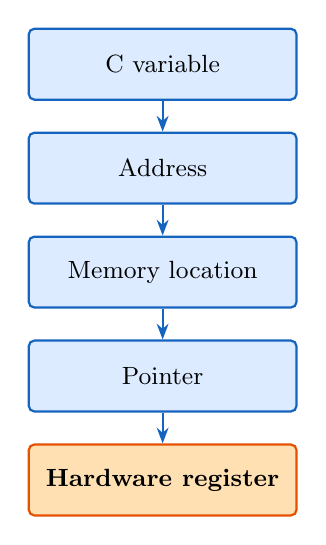
\begin{tikzpicture}[x=10mm, y=11mm]
        \node[blk,    minimum width=34mm] (var)  at (0,2.4)  {C variable};
        \node[blk,    minimum width=34mm] (addr) at (0,1.2) {Address};
        \node[blk,    minimum width=34mm] (loc)  at (0,0)    {Memory location};
        \node[blk,    minimum width=34mm] (ptr)  at (0,-1.2){Pointer};
        \node[cpublk, minimum width=34mm] (reg)  at (0,-2.4) {Hardware register};
        \foreach \x/\y in {var/addr, addr/loc, loc/ptr, ptr/reg}{\draw[flow] (\x) -- (\y);}
    \end{tikzpicture}
    \end{center}
\end{frame}

%===============================================================================
\section{Types and Qualifiers}
%===============================================================================

\begin{frame}{Fixed-Width Types}
    \leavevmode
    {\small In desktop C, \texttt{int} is a reasonable default choice.
    In embedded C it is a \alert{hazard}, because the C standard does
    not fix its width --- and every access we just wrote depends on
    knowing the exact width.}

    \vspace{2mm}
    \begin{center}
    {\small
    \striped
    \begin{tabular}{@{}l l l l@{}}
        \toprule
        \textbf{Type} & \textbf{Width} & \textbf{Sign} & \textbf{Range} \\
        \midrule
        \texttt{uint8\_t}  & 8-bit  & Unsigned & 0 to 255 \\
        \texttt{int8\_t}   & 8-bit  & Signed   & $-128$ to $127$ \\
        \texttt{uint16\_t} & 16-bit & Unsigned & 0 to 65{,}535 \\
        \texttt{uint32\_t} & 32-bit & Unsigned & 0 to 4{,}294{,}967{,}295 \\
        \texttt{int32\_t}  & 32-bit & Signed   & $\pm 2{,}147{,}483{,}647$ \\
        \bottomrule
    \end{tabular}}
    \end{center}

    \vspace{2mm}
    \begin{block}{Two rules}
        \alert{Match the hardware}: a 32-bit register is always
        \texttt{uint32\_t}. A 12-bit ADC result fits in
        \texttt{uint16\_t}.

        \vspace{1mm}
        \alert{Then save space}, but watch for overflow. If two
        \texttt{uint8\_t} values add up to more than 255, the result
        gets cut off. Add them into a wider type instead.
    \end{block}
\end{frame}

\begin{frame}{Data Sizes and Alignment}
    \leavevmode
    {\small A pointer's type does not only set the step size in pointer
    arithmetic. It also sets how many bytes one access reads or writes,
    and where that access is allowed to start.}

    \begin{columns}[T]
    \begin{column}{.5\textwidth}
        {\small
        \striped
        \begin{tabular}{@{}l l l l@{}}
            \toprule
            \textbf{Name} & \textbf{Bits} & \textbf{Bytes} & \textbf{C type} \\
            \midrule
            Byte     & 8  & 1 & \texttt{uint8\_t} \\
            Halfword & 16 & 2 & \texttt{uint16\_t} \\
            Word     & 32 & 4 & \texttt{uint32\_t} \\
            \bottomrule
        \end{tabular}}

        \vspace{3mm}
        {\small A word starting at \texttt{0x20000000} occupies
        \texttt{0x20000000}--\texttt{0x20000003}. The next word starts at
        \texttt{0x20000004}.}
    \end{column}
    \begin{column}{.46\textwidth}
        \textbf{Alignment}
        {\small
        \begin{itemize}\itemsep1pt
            \item Word access should be at a \alert{multiple of 4}
            \item Halfword access at an \alert{even} address
            \item Aligned accesses are generally more efficient.
                  Misaligned ones are slower, or cause a fault
        \end{itemize}}
    \end{column}
    \end{columns}

    \vspace{3mm}
    \begin{block}{Why every STM32 register offset advances by 4}
        Each peripheral register is one \alert{word}. When a datasheet
        shows offsets \texttt{0x00}, \texttt{0x04}, \texttt{0x08}, this
        is why: each one sits 4 bytes further than the last.
    \end{block}
\end{frame}

\begin{frame}{When Memory Can Change Without C Changing It}
    \leavevmode
    {\small Every C program relies on one basic assumption, so basic
    that we rarely notice it: \emph{a variable's value changes only
    when your code changes it.}}

    \vspace{2mm}
    {\small
    \begin{enumerate}\itemsep2pt
        \item \textbf{An ordinary variable} always obeys this rule.
              Nothing else can touch it between two reads.
        \item \textbf{The compiler relies on this too}: it may read a
              value \alert{once}, store it in a register, and reuse
              that register on every later access.
        \item \textbf{A hardware register breaks this assumption}. It
              is memory-mapped, so C reaches it through an ordinary
              pointer --- but it changes because a conversion
              finished, or a timer overflowed, not because of a C
              assignment.
        \item \textbf{A variable shared with an ISR} has the same
              problem: to the main program, a flag the ISR sets seems
              to change with no matching write.
        \item \textbf{\texttt{volatile} is the fix}: it tells the
              compiler to re-read this address every time, and to
              perform every write, in order, with none skipped.
    \end{enumerate}}

    \vspace{2mm}
    \begin{block}{The statement to remember}
        \texttt{volatile} tells the compiler a value may change
        \alert{outside the current sequence of C statements}. Hardware
        registers are just the most common reason this happens in
        embedded code.
    \end{block}
\end{frame}

\begin{frame}[fragile]{\texttt{volatile} in Practice}
    \leavevmode
\begin{lstlisting}[language=C, basicstyle=\ttfamily\normalsize]
volatile uint32_t *status = (volatile uint32_t *)0x40011000;
while ((*status & 1) == 0) {
    // Without volatile the compiler reads the address once, caches it,
    // and this loop never terminates no matter what the hardware does.
}
\end{lstlisting}

    \vspace{3mm}
    \begin{block}{The rule}
        \emph{Every pointer to a hardware register, and every variable
        shared with an interrupt handler, must be
        \alert{\texttt{volatile}}.}
    \end{block}

    \vspace{2mm}
    {\small Chapter 9 uses this same keyword for a different situation:
    an ISR talks to the main loop using nothing more than a flag.}
\end{frame}

\begin{frame}[fragile]{A Brief Aside: \texttt{const}}
    \leavevmode
    \texttt{const} is a promise: the program will not change this
    object. The practical benefit is \alert{placement}: a
    \texttt{const} array can live in Flash instead of SRAM, so it
    costs no scarce RAM.

    \vspace{3mm}
\begin{lstlisting}[language=C, basicstyle=\ttfamily\normalsize]
const uint8_t sine_table[256] = {
    128, 131, 134, /* ... */
};  // lives in Flash
\end{lstlisting}

    \vspace{3mm}
    {\small That is all there is to \texttt{const}. It says nothing
    about \emph{when} a value can change, which is exactly the question
    \texttt{volatile} answers.}
\end{frame}

%===============================================================================
\section{From Pointer to Instruction}
%===============================================================================

\begin{frame}{What a Pointer Becomes}
    \leavevmode
    Every pointer operation compiles into one of exactly \alert{two}
    instructions: a \textbf{load} or a \textbf{store}.

    \vspace{2mm}
    \begin{center}
    {\small
    \striped
    \begin{tabular}{@{}l l R{.44\textwidth}@{}}
        \toprule
        \textbf{C} & \textbf{Instruction} & \textbf{What happens} \\
        \midrule
        \texttt{v = *p;}       & \texttt{LDR R0, [R1]}      & Read the word at the address in R1 \\
        \texttt{*p = v;}       & \texttt{STR R0, [R1]}      & Write R0 to the address in R1 \\
        \texttt{v = p[2];}     & \texttt{LDR R0, [R1, \#8]} & Read the word 8 bytes past R1 \\
        \texttt{c = *bytePtr;} & \texttt{LDRB R0, [R1]}     & Read one \emph{byte}, zero-filled \\
        \bottomrule
    \end{tabular}}
    \end{center}

    \vspace{2mm}
    \begin{block}{A dereference is a direction}
        On the \alert{right} of an assignment, it is a \textbf{load}.
        On the \alert{left}, it is a \textbf{store}. The pointer
        itself is just a 32-bit number in a register, supplying the
        address.
    \end{block}

    \vspace{2mm}
    {\small This is the mechanical end of the story: a pointer
    dereference is not an abstraction, it \emph{is} one of these two
    instructions.}
\end{frame}

\begin{frame}{Where Variables Live}
    \leavevmode
    {\small A pointer is an address --- but who decides \emph{which}
    address a variable gets? \textbf{Must understand:} the stack,
    global/static storage, Flash, SRAM. \textbf{Should understand:} the
    heap.}

    \vspace{1mm}
    \begin{columns}[T]
    \begin{column}{.4\textwidth}
        \begin{center}
\begin{tikzpicture}[node distance=0pt]
	% ---- Flash: a separate block on the left ----
	\node[memblk, minimum width=22mm, minimum height=28mm, align=center,
	font=\scriptsize] (flash) {code\\[1.5mm]\texttt{const}\\data};
	\node[lbl, font=\scriptsize\bfseries, above=1.5mm of flash] {Flash};

	% ---- SRAM: one contiguous block, divided into regions ----
	\node[cpublk, minimum width=22mm, minimum height=7mm, font=\scriptsize,
	right=14mm of flash.north east, anchor=north west] (stack) {stack};
	\node[blk, draw=Gray!50, fill=Gray!8, minimum width=22mm, minimum height=9mm,
	font=\scriptsize, text=Gray, below=of stack] (free) {free space};
	\node[blk, minimum width=22mm, minimum height=6mm, font=\scriptsize,
	below=of free] (heap) {heap};
	\node[blk, minimum width=22mm, minimum height=6mm, align=center,
	font=\scriptsize, below=of heap] (glob) {globals /\\statics};
	\node[lbl, font=\scriptsize\bfseries, above=1.5mm of stack] {SRAM};

	% ---- growth directions, outside the right edge ----
	\draw[-{Stealth[length=1.8mm]}, draw=primary, thick]
	([xshift=-4mm]stack.south east) -- ([xshift=-4mm, yshift=-4mm]stack.south east);
	\draw[-{Stealth[length=1.8mm]}, draw=secondary, thick]
	([xshift=-4mm]heap.north east) -- ([xshift=-4mm, yshift=4mm]heap.north east);
	\end{tikzpicture}
        \end{center}
    \end{column}
    \begin{column}{.56\textwidth}
        \textbf{The stack}
        {\small
        \begin{itemize}\itemsep1pt
            \item Locals, arguments beyond the first four, saved registers,
                  return addresses
            \item Managed automatically by \alert{SP (R13)}
            \item Grows \alert{downward} from the top of SRAM
            \item Chapter 7 builds an entire chapter on it
        \end{itemize}}

        \vspace{1mm}
        \textbf{The heap}
        {\small
        \begin{itemize}\itemsep1pt
            \item Gives memory through \texttt{malloc()}, freed by
                  \texttt{free()}
            \item \alert{Usually avoided} in bare-metal work: it can
                  fail at runtime when memory fragments, and its
                  timing is not predictable
            \item Almost no example in this book calls \texttt{malloc}
        \end{itemize}}
    \end{column}
    \end{columns}

    \vspace{2mm}
    \begin{block}{Stack overflow --- a classic embedded failure}
        The downward-growing stack can collide with the upward-growing
        global data. This \alert{silently corrupts variables}. The
        usual causes are deep recursion and large local arrays.
    \end{block}
\end{frame}

\begin{frame}{Summary}
	\begin{columns}[c]
		\begin{column}{.62\textwidth}
			\begin{center}
				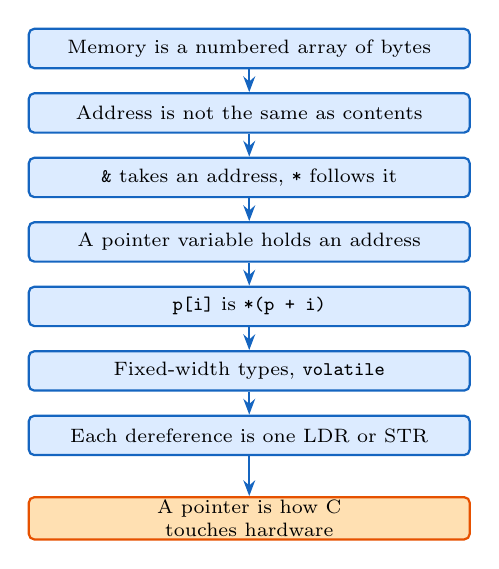
\begin{tikzpicture}[x=10mm, y=7.8mm]
					\node[blk, minimum width=56mm, minimum height=5.0mm, inner sep=1.2pt, font=\scriptsize] (n0) at (0,0.00) {Memory is a numbered array of bytes};
					\node[blk, minimum width=56mm, minimum height=5.0mm, inner sep=1.2pt, font=\scriptsize] (n1) at (0,-1.05) {Address is not the same as contents};
					\node[blk, minimum width=56mm, minimum height=5.0mm, inner sep=1.2pt, font=\scriptsize] (n2) at (0,-2.10) {\texttt{\&} takes an address, \texttt{*} follows it};
					\node[blk, minimum width=56mm, minimum height=5.0mm, inner sep=1.2pt, font=\scriptsize] (n3) at (0,-3.15) {A pointer variable holds an address};
					\node[blk, minimum width=56mm, minimum height=5.0mm, inner sep=1.2pt, font=\scriptsize] (n4) at (0,-4.20) {\texttt{p[i]} is \texttt{*(p + i)}};
					\node[blk, minimum width=56mm, minimum height=5.0mm, inner sep=1.2pt, font=\scriptsize] (n5) at (0,-5.25) {Fixed-width types, \texttt{volatile}};
					\node[blk, minimum width=56mm, minimum height=5.0mm, inner sep=1.2pt, font=\scriptsize] (n6) at (0,-6.30) {Each dereference is one LDR or STR};
					\node[cpublk, minimum width=56mm, minimum height=5.0mm, inner sep=1.2pt, font=\scriptsize, align=center] (n7) at (0,-7.65) {A pointer is how C\\touches hardware};
					\foreach \a/\b in {0/1,1/2,2/3,3/4,4/5,5/6,6/7}{\draw[flow] (n\a) -- (n\b);}
				\end{tikzpicture}
			\end{center}
		\end{column}
		\begin{column}{.34\textwidth}
			{\scriptsize
				\textbf{Terminology covered}\\[1mm]
				\begin{itemize}
					\item Address, byte, halfword, word
					\item Pointer, \texttt{\&}, \texttt{*}
					\item Fixed-width types
					\item \texttt{const}, \texttt{volatile}
				\end{itemize}
				\vspace{3mm}
				\textbf{Next: Chapter 4}\\[1mm]
				\emph{Embedded C and CMSIS}\\[1mm]
				We use this mechanism to turn on a real LED.}
		\end{column}
	\end{columns}
\end{frame}

\end{document}
